\section{Lush Decision Studio: Modelo de Soporte para Decisiones}\label{cap:decision}

Lush Decision Studio constituye el núcleo distintivo para la materia. La gestión transaccional responde cuánto se cobró y cuánto se debe liquidar; el módulo DSS responde qué alternativas son posibles, qué resultado podría generar cada una, bajo qué hipótesis y con qué riesgos. Se organiza en cinco funciones implementables y dos módulos experimentales. Toda cifra derivada de un supuesto se rotulará como simulación y se mantendrá separada de los registros operativos.


\subsection{Tipos de decisiones y responsables}

\vspace{8pt}{\small\setstretch{1.0}
\begin{longtable}{>{\raggedright\arraybackslash}p{0.3333\dimexpr\linewidth-6\tabcolsep\relax}>{\raggedright\arraybackslash}p{0.3333\dimexpr\linewidth-6\tabcolsep\relax}>{\raggedright\arraybackslash}p{0.3333\dimexpr\linewidth-6\tabcolsep\relax}}
\caption{Matriz de decisiones que puede apoyar el sistema y responsabilidad de aprobación}\label{tab:dss_9}\\
\toprule
\textbf{Decisión} & \textbf{Entradas necesarias} & \textbf{Salida y responsable} \\
\midrule\endfirsthead
\toprule
\textbf{Decisión} & \textbf{Entradas necesarias} & \textbf{Salida y responsable} \\
\midrule\endhead
\bottomrule\endfoot
\bottomrule\endlastfoot
Modificar descuentos & Lista de precios, regla vigente, costo variable, volumen hipotético & Comparación de escenarios; aprueba administradora \\
Revisar precio de un servicio & Costo directo, comisión, duración e historial de ventas & Contribución estimada y sensibilidad; aprueba administradora \\
Analizar política de comisión & Precio de lista/cobrado y reglas históricas & Simulación de impacto; requiere acuerdo y autorización \\
Revisar cierre de caja & Ventas, métodos de pago, devoluciones, ajustes & Alertas de diferencias; resuelve administradora \\
Programar capacidad & Duración del servicio y horas disponibles & Alternativas de asignación; fase experimental \\
\end{longtable}}
\nota{Propuesta de diseño.}

El DSS ofrecerá sugerencias, nunca cambios automáticos en remuneraciones o condiciones laborales. Antes de interpretar como utilidad una diferencia, el motor distinguirá contribución de costos directos, gastos fijos no distribuidos e impuestos. Si falta un costo necesario, mostrará la limitación.


\subsection{Lush Decision Studio y sus cinco capacidades principales}

\subsubsection{Análisis de contribución por servicio}

Para cada tipo de servicio se registrará, cuando sea posible, un costo variable estimado de materiales, la comisión vigente y la duración. El indicador principal será contribución por servicio = precio realmente cobrado − comisión reconocida − costos variables directos. El resultado no equivale automáticamente a utilidad neta del negocio. Los costos tendrán fecha de vigencia y fuente documentada.


\subsubsection{Simulación What-If}

La administradora creará un escenario base y alternativas cambiando precio de lista, tasa de descuento, comisión, costos directos y cantidad prevista de servicios. Cada escenario almacenará sus parámetros, fecha, responsable y carácter supuesto/observado. El sistema presentará ingresos, comisiones, materiales, contribución agregada y punto de equilibrio de volumen.


\subsubsection{Comparación multicriterio}

Las alternativas podrán evaluarse según contribución, liquidez, riesgo y facilidad operativa. Se usarán escalas explícitas; los pesos deberán sumar 100~\%. La puntuación exploratoria se calculará con una suma ponderada de puntuaciones normalizadas y se acompañará de pruebas de sensibilidad y restricciones mínimas.


\subsubsection{Recomendaciones explicables}

El motor propondrá cursos de acción a partir de resultados ya calculados, señalará cuáles criterios favorecen cada opción y advertirá sobre incertidumbre, datos incompletos o supuestos sensibles. Lush Insight podrá redactar una explicación en lenguaje natural, pero no recalculará importes con texto generado ni determinará la alternativa ganadora por intuición.


\subsubsection{Historial y evaluación de decisiones}

Al aprobarse una alternativa se guardarán motivo, responsable, supuestos, resultados esperados, fecha de revisión y resultado observado. Esta bitácora permitirá diferenciar una recomendación emitida de una decisión efectivamente aplicada y medir la precisión de su hipótesis, sin atribuir automáticamente efectos causales.


\subsection{Variables de decisión, restricciones y ecuaciones}

\vspace{8pt}{\small\setstretch{1.0}
\begin{longtable}{>{\raggedright\arraybackslash}p{0.3333\dimexpr\linewidth-6\tabcolsep\relax}>{\raggedright\arraybackslash}p{0.3333\dimexpr\linewidth-6\tabcolsep\relax}>{\raggedright\arraybackslash}p{0.3333\dimexpr\linewidth-6\tabcolsep\relax}}
\caption{Variables y fórmulas de simulación}\label{tab:dss_10}\\
\toprule
\textbf{Variable} & \textbf{Símbolo} & \textbf{Interpretación / regla} \\
\midrule\endfirsthead
\toprule
\textbf{Variable} & \textbf{Símbolo} & \textbf{Interpretación / regla} \\
\midrule\endhead
\bottomrule\endfoot
\bottomrule\endlastfoot
Precio de lista & P & Valor de catálogo vigente para el servicio \\
Descuento & d & Proporción entre 0 y 1 autorizada por política \\
Precio cobrado & R & P × (1 − d); ajustar si existen promociones combinadas \\
Tasa de comisión & c & Proporción definida por política con vigencia \\
Base de comisión & B & P o R, según regla aprobada y snapshot histórico \\
Materiales variables & M & Estimación directa por servicio; puede no estar disponible \\
Contribución unitaria & U & R − (c × B) − M \\
Cantidad de servicios & Q & Observada o supuesta según tipo de escenario \\
Contribución total & CT & U × Q, bajo hipótesis de costos unitarios constantes \\
\end{longtable}}
\nota{El sistema usa importes decimales, no coma flotante para dinero.}

Para dos alternativas A y B con contribución unitaria positiva y costos comparables, el volumen mínimo para que B iguale la contribución de A se estima como $Q_B$ = ($U_A$ × $Q_A$) / $U_B$. Esta fórmula omite efectos no lineales y restricciones de capacidad: el motor debe comprobarlos antes de presentar una equivalencia como factible. Las comisiones históricas nunca se recalculan retroactivamente a partir de una nueva política.


\subsection{Caso trabajado: comparación de descuentos en un servicio}

Ejemplo exclusivamente didáctico. Se supone un servicio con precio de lista Bs~120, tasa de comisión del 35~\% sobre el precio de lista y costo variable de materiales Bs~20. Para un mes hipotético se comparan tres políticas: A sin descuento, B con 5~\% y C con 10~\%. Los volúmenes 100, 110 y 130 son supuestos deliberados para ilustrar decisiones; no representan una predicción ni demanda observada en Lush Beauty.


\vspace{8pt}{\footnotesize\setstretch{1.0}
\begin{longtable}{>{\raggedright\arraybackslash}p{0.1429\dimexpr\linewidth-14\tabcolsep\relax}>{\raggedright\arraybackslash}p{0.1429\dimexpr\linewidth-14\tabcolsep\relax}>{\raggedright\arraybackslash}p{0.1429\dimexpr\linewidth-14\tabcolsep\relax}>{\raggedright\arraybackslash}p{0.1429\dimexpr\linewidth-14\tabcolsep\relax}>{\raggedright\arraybackslash}p{0.1429\dimexpr\linewidth-14\tabcolsep\relax}>{\raggedright\arraybackslash}p{0.1429\dimexpr\linewidth-14\tabcolsep\relax}>{\raggedright\arraybackslash}p{0.1429\dimexpr\linewidth-14\tabcolsep\relax}}
\caption{Simulación ilustrativa de tres decisiones comerciales; todos los volúmenes son hipotéticos}\label{tab:dss_11}\\
\toprule
\textbf{Escenario} & \textbf{Cobro unit.} & \textbf{Comisión} & \textbf{Materiales} & \textbf{Contrib./serv.} & \textbf{Q supuesto} & \textbf{Contrib. mes} \\
\midrule\endfirsthead
\toprule
\textbf{Escenario} & \textbf{Cobro unit.} & \textbf{Comisión} & \textbf{Materiales} & \textbf{Contrib./serv.} & \textbf{Q supuesto} & \textbf{Contrib. mes} \\
\midrule\endhead
\bottomrule\endfoot
\bottomrule\endlastfoot
A. Sin descuento & Bs~120 & Bs~42 & Bs~20 & Bs~58 & 100 & Bs~5.800 \\
B. Descuento 5~\% & Bs~114 & Bs~42 & Bs~20 & Bs~52 & 110 & Bs~5.720 \\
C. Descuento 10~\% & Bs~108 & Bs~42 & Bs~20 & Bs~46 & 130 & Bs~5.980 \\
\end{longtable}}

La alternativa C arroja la mayor contribución mensual bajo el supuesto de 130 servicios. No obstante, para igualar los Bs~5.800 de A con una contribución de Bs~46 por servicio, C necesitaría al menos 127 servicios completos (5.800 / 46 ≈ 126,09), es decir, aproximadamente 27~\% más que los 100 servicios de A. Con una demanda menor podría ser inferior. La comparación no demuestra que un descuento atraiga clientas; esa relación debe estudiarse por separado.


\begin{figure}[H]
\caption{Contribución hipotética por alternativa}\label{fig:dss_4}
\centering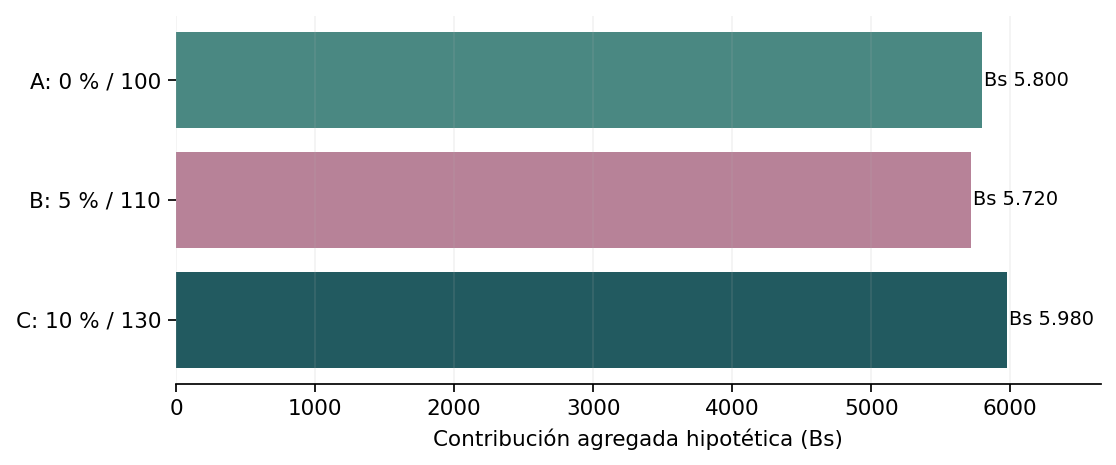
\includegraphics[width=0.9\linewidth]{img/fig_contribucion.png}
\end{figure}
\nota{Los volúmenes de servicios son supuestos, no pronósticos.}

\subsection{Matriz de alternativas, criterios y sensibilidad}

Como primer mecanismo de selección, el equipo desarrollará una matriz de puntuación ponderada exploratoria. Se proponen cuatro criterios con puntuaciones del 1 al 5 (5 representa mejor desempeño), normalizadas antes de sumar. Los pesos son una configuración de ejemplo que requiere validación de la propietaria. Los valores cualitativos de riesgo y facilidad deben justificarse con evidencia o juicio explícito, sin aparecer como resultados objetivos.


\vspace{8pt}{\small\setstretch{1.0}
\begin{longtable}{>{\raggedright\arraybackslash}p{0.2000\dimexpr\linewidth-10\tabcolsep\relax}>{\raggedright\arraybackslash}p{0.2000\dimexpr\linewidth-10\tabcolsep\relax}>{\raggedright\arraybackslash}p{0.2000\dimexpr\linewidth-10\tabcolsep\relax}>{\raggedright\arraybackslash}p{0.2000\dimexpr\linewidth-10\tabcolsep\relax}>{\raggedright\arraybackslash}p{0.2000\dimexpr\linewidth-10\tabcolsep\relax}}
\caption{Matriz ponderada de ejemplo; la puntuación es ilustrativa, dependiente de los criterios y pesos definidos}\label{tab:dss_12}\\
\toprule
\textbf{Criterio} & \textbf{Peso} & \textbf{A} & \textbf{B} & \textbf{C} \\
\midrule\endfirsthead
\toprule
\textbf{Criterio} & \textbf{Peso} & \textbf{A} & \textbf{B} & \textbf{C} \\
\midrule\endhead
\bottomrule\endfoot
\bottomrule\endlastfoot
Contribución mensual esperada & 40~\% & 4 & 3 & 5 \\
Liquidez y previsibilidad & 25~\% & 5 & 4 & 3 \\
Riesgo de demanda & 20~\% & 5 & 4 & 2 \\
Facilidad de operación & 15~\% & 5 & 4 & 3 \\
Puntaje ponderado & 100~\% & 4,60 & 3,60 & 3,60 \\
\end{longtable}}

Con la ponderación del ejemplo, A ocupa el primer lugar por su menor incertidumbre, aunque C genere más contribución bajo el escenario de volumen asumido. Si el peso de la contribución pasa del 40~\% al 75~\% y se reducen proporcionalmente los demás criterios, C podría pasar a ser preferida. Esta sensibilidad deberá calcularse automáticamente y visualizarse, no ocultarse. Cuando existan criterios de exclusión (por ejemplo, incumplimiento de límites aprobados de descuentos), las alternativas no elegibles se descartan antes del ranking.


La matriz de pesos constituye una herramienta didáctica de análisis multicriterio; no debe presentarse como aplicación exhaustiva de MCDA. La evaluación posterior puede incorporar valoración de rangos, compensaciones, incertidumbre y revisión de escalas conforme a guías especializadas.


\subsection{Motor prescriptivo y protocolo de explicación}

Cada recomendación expondrá seis elementos obligatorios: problema de decisión; alternativas y criterios; datos de procedencia; operaciones realizadas; supuestos y límites; y alternativa sugerida con necesidad de aprobación. Si faltan precios vigentes, costos directos o cantidades confiables, el motor mostrará “evidencia insuficiente” y propondrá obtener la información, no inventar una conclusión. La capa generativa solo podrá traducir una estructura de resultados ya calculados por el backend.


\vspace{8pt}{\small\setstretch{1.0}
\begin{longtable}{>{\raggedright\arraybackslash}p{0.3333\dimexpr\linewidth-6\tabcolsep\relax}>{\raggedright\arraybackslash}p{0.3333\dimexpr\linewidth-6\tabcolsep\relax}>{\raggedright\arraybackslash}p{0.3333\dimexpr\linewidth-6\tabcolsep\relax}}
\caption{Trazabilidad de una recomendación desde la información hasta su aprobación}\label{tab:dss_13}\\
\toprule
\textbf{Entrada} & \textbf{Proceso controlado} & \textbf{Salida} \\
\midrule\endfirsthead
\toprule
\textbf{Entrada} & \textbf{Proceso controlado} & \textbf{Salida} \\
\midrule\endhead
\bottomrule\endfoot
\bottomrule\endlastfoot
Movimientos y catálogo & Consulta agregada y autorizada & Indicadores comprobables \\
Escenarios y parámetros & Motor Decimal y simulaciones & Tabla comparativa, umbrales \\
Criterios y pesos & Matriz y sensibilidad & Orden condicional de alternativas \\
Datos, límites y resultados & Plantilla + explicación LLM opcional & Texto con trazas y advertencias \\
Aprobación humana & Bitácora de decisión & Registro y fecha de revisión \\
\end{longtable}}

\subsection{Proyección de caja y análisis de riesgo}

La proyección de caja será distinta a la rentabilidad: partirá de saldos conciliados, cobros efectivamente disponibles, pagos previstos y fechas de vencimiento. La propuesta inicial admite escenarios bajo, base y alto basados en rangos editables. Los pronósticos estadísticos quedan condicionados a contar con un historial temporal suficiente y a evaluar el error de predicción mediante separación temporal de datos (scikit-learn Developers, s. f.-b). El sistema no afirmará capacidad predictiva hasta superar esa validación.


Un tablero de riesgo puede mostrar el efecto de variaciones del volumen de servicios, materiales o descuentos. En esta fase se recomienda análisis de escenarios y sensibilidad determinista antes que simulaciones probabilísticas complejas, porque las distribuciones de probabilidad requerirían justificación adicional.


\subsection{Optimización de capacidad como funcionalidad experimental}

Si el salón registra duración promedio y disponibilidad voluntariamente autorizada por cada especialista, un módulo experimental puede plantear una optimización: maximizar contribución esperada sujeta a horas disponibles y restricciones operativas. Se propone explorar programación lineal mediante SciPy (función linprog) o programación entera cuando se necesiten cantidades discretas. El resultado sería una alternativa de planificación, no una agenda automática ni una instrucción rígida para las trabajadoras.


Modelo orientativo: maximizar $\sum$ $U_i$ × $x_i$ sujeto a $\sum$ $t_i$ × $x_i$ $\leq$ H, $x_i$ $\geq$ 0 y, cuando corresponda, valores enteros. Esta simplificación no captura preferencias de clientas, diferencias de habilidades ni variaciones reales de demanda; por ello solo se incluirá si los datos permiten explicar sus límites.


\subsection{Registro y aprendizaje de las decisiones}

\vspace{8pt}{\small\setstretch{1.0}
\begin{longtable}{>{\raggedright\arraybackslash}p{0.5000\dimexpr\linewidth-4\tabcolsep\relax}>{\raggedright\arraybackslash}p{0.5000\dimexpr\linewidth-4\tabcolsep\relax}}
\caption{Modelo mínimo de auditoría de decisiones (registro propuesto)}\label{tab:dss_14}\\
\toprule
\textbf{Campo} & \textbf{Descripción} \\
\midrule\endfirsthead
\toprule
\textbf{Campo} & \textbf{Descripción} \\
\midrule\endhead
\bottomrule\endfoot
\bottomrule\endlastfoot
decision\_id / salon\_id & Identificación y aislamiento de cada decisión \\
problema / responsable & Cuestión planteada y persona que aprueba \\
alternativas / criterios / pesos & Instantánea de opciones y modelo usado \\
supuestos / fuente de datos & Origen, versión y confiabilidad de la información \\
recomendación / decisión final & Propuesta del sistema y elección efectiva \\
resultado esperado / fecha de revisión & Meta verificable y periodo de seguimiento \\
resultado observado / comentario & Evidencia posterior y explicación de diferencias \\
\end{longtable}}

El historial servirá para mejorar la calidad del proceso, no para automatizar atribuciones causales. Por ejemplo, si después de un descuento aumentan las ventas, el sistema registrará la coincidencia temporal pero no concluirá que el descuento causó el cambio sin evidencia apropiada.


\begin{figure}[H]
\caption{Ciclo propuesto para transformar datos financieros en decisiones humanas revisables}\label{fig:dss_5}
\centering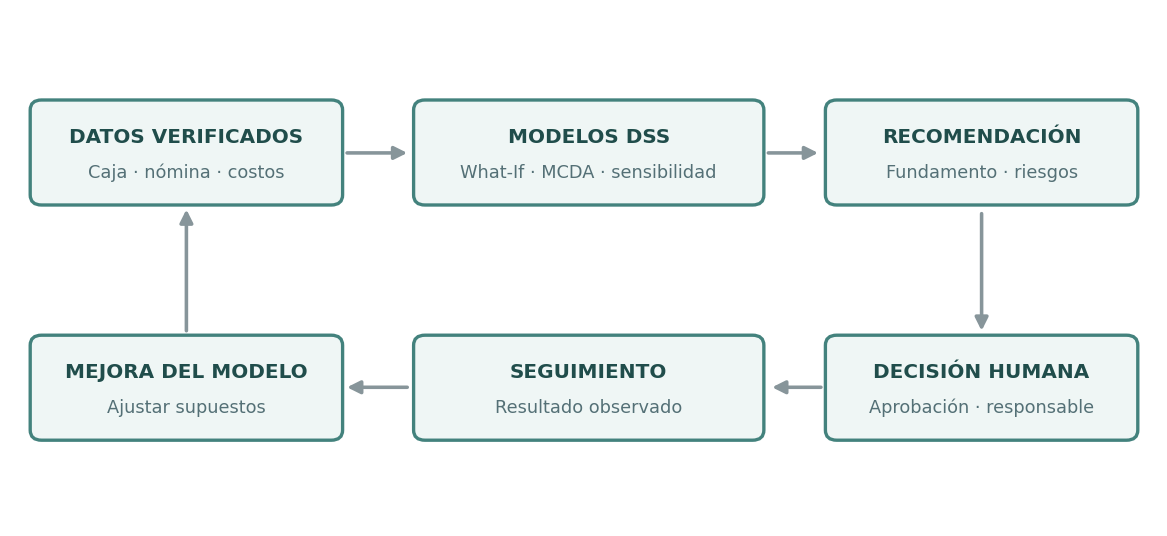
\includegraphics[width=0.9\linewidth]{img/fig_ciclo_decision.png}
\end{figure}
\nota{Elaboración propia.}

\subsection{Requisitos funcionales adicionales del DSS}

\vspace{8pt}{\small\setstretch{1.0}
\begin{longtable}{>{\raggedright\arraybackslash}p{0.3333\dimexpr\linewidth-6\tabcolsep\relax}>{\raggedright\arraybackslash}p{0.3333\dimexpr\linewidth-6\tabcolsep\relax}>{\raggedright\arraybackslash}p{0.3333\dimexpr\linewidth-6\tabcolsep\relax}}
\caption{Requisitos del módulo de soporte para decisiones; deben validarse con el negocio}\label{tab:dss_15}\\
\toprule
\textbf{Código} & \textbf{Requisito verificable} & \textbf{Prioridad} \\
\midrule\endfirsthead
\toprule
\textbf{Código} & \textbf{Requisito verificable} & \textbf{Prioridad} \\
\midrule\endhead
\bottomrule\endfoot
\bottomrule\endlastfoot
DSS-01 & Calcular contribución por servicio con costos directos configurables y trazables & MVP \\
DSS-02 & Crear, editar y comparar al menos tres escenarios sin modificar datos reales & MVP \\
DSS-03 & Aplicar matriz de criterios, pesos normalizados y umbrales de exclusión & MVP \\
DSS-04 & Realizar sensibilidad ante variaciones de pesos y demanda & MVP \\
DSS-05 & Producir recomendación con datos, supuestos, cálculos y advertencias & MVP \\
DSS-06 & Solicitar aprobación humana antes de aplicar una decisión & MVP \\
DSS-07 & Guardar decisiones, resultados esperados y revisión posterior & MVP \\
DSS-08 & Proyectar saldo de caja con escenarios de entradas y salidas & Extensión \\
DSS-09 & Optimizar capacidad usando restricciones de tiempo y disponibilidad & Experimental \\
DSS-10 & Entrenar y validar pronósticos con historial suficiente & Futuro \\
\end{longtable}}
